\documentclass[11pt]{article}
\usepackage[a4paper,margin=2cm]{geometry}
\usepackage[brazilian]{babel}
\usepackage{caption}
\usepackage{subcaption}
\usepackage[T1]{fontenc}
\linespread{1.3}
\parskip=12pt
\parindent=0pt
\usepackage{enumerate}
\usepackage{amsfonts}
\usepackage{amsmath}
\usepackage{amsfonts}
\usepackage{graphicx}

\begin{document}
	\begin{center}
		{\LARGE{\textbf{Lista 3 - Macroeconomia III 2017}}}\\
		\vspace{0.2cm}
		Alunos: Alexandre Machado e Raul Guarini\\
		Monitora: K�tia Alves\\
		\today
	\end{center}
	
\section*{Exerc�cio 1}

Come�amos com $\underline{a} = -2$ e $q = 1$ como chute inicial. Consideramos um grid para o ativo de 100 pontos em cada exerc�cio.A primeira itera��o gerou as seguintes fun��o valor e fun��o pol�tica:

\begin{center}
	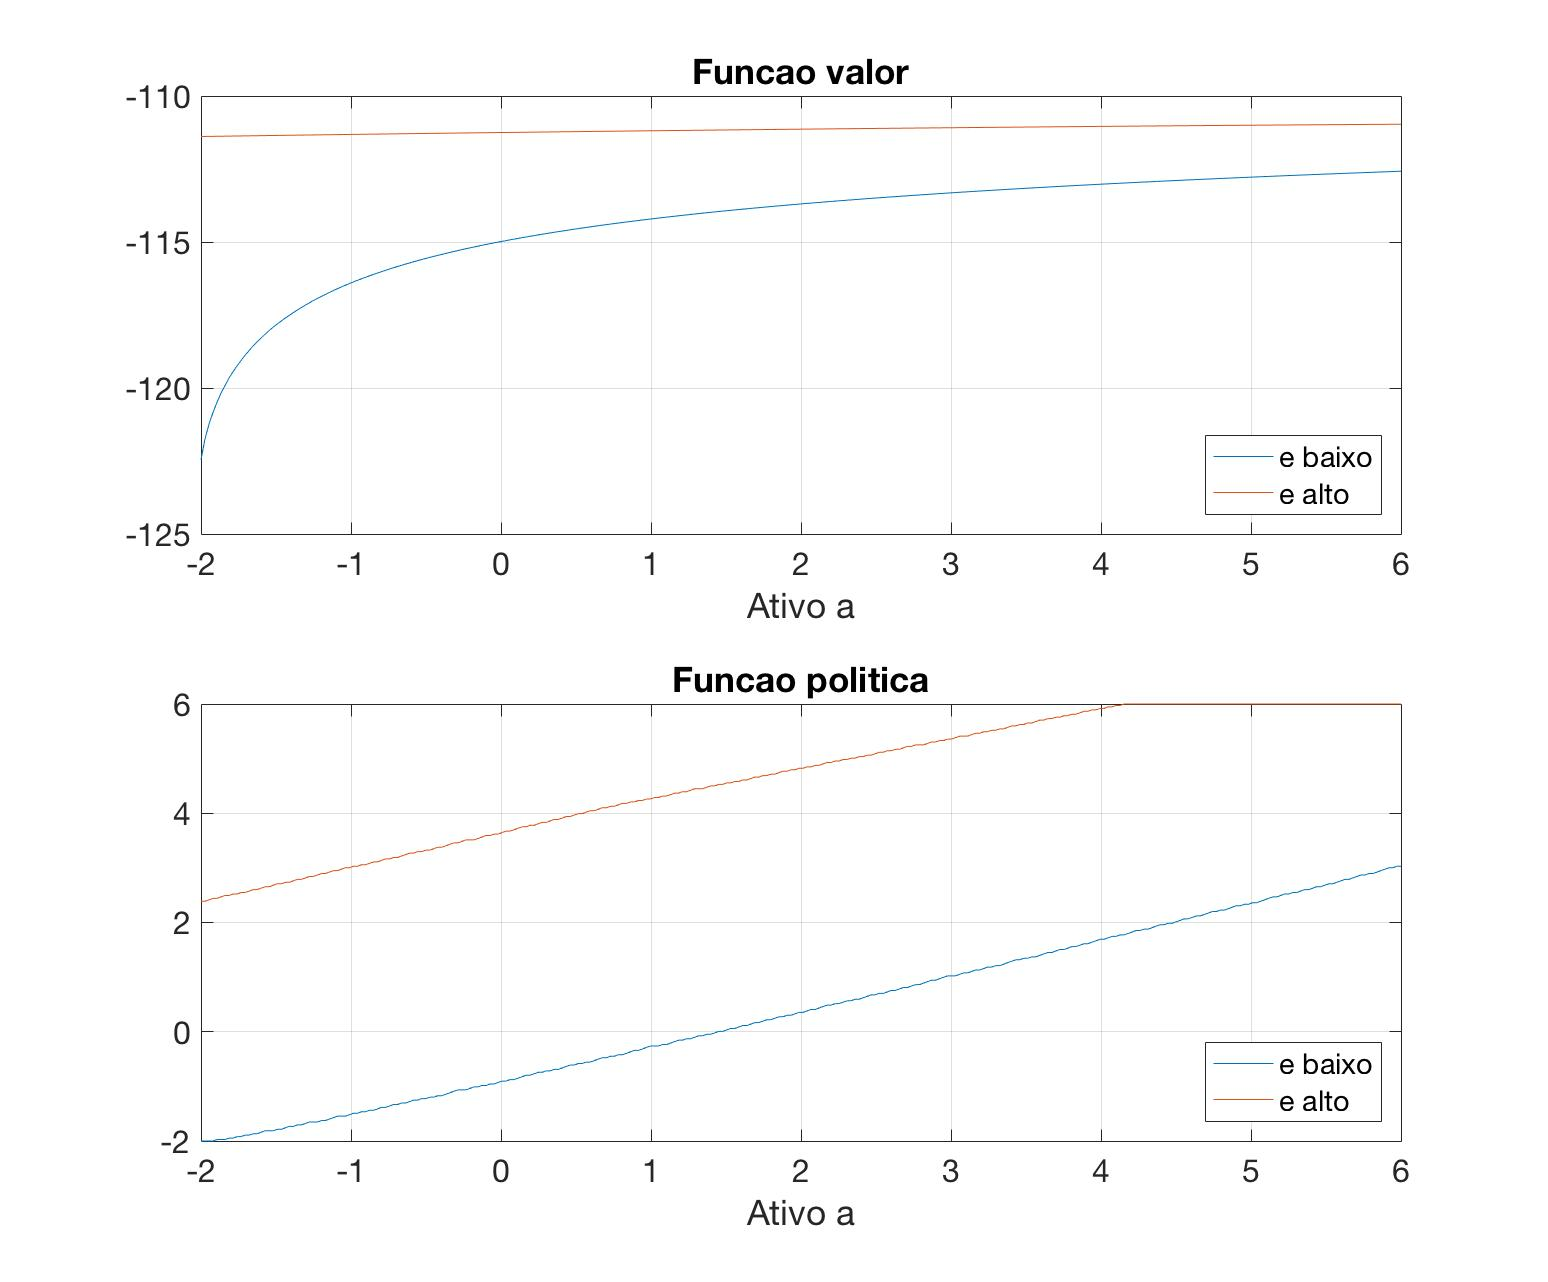
\includegraphics[scale = 0.25]{init_valuefunction}
\end{center}

O c�digo referente a este exerc�cio � est� no arquivo \textit{q1\_ae.m}. Como esperado, ao calcular as distribui��es invariantes pelo m�todo iterativo e pelo m�todo do maior autovalor tivemos os mesmos resultados.

Agora, ajustando o valor de $q$ para alcan�ar market clearing num�rico (c�digo dispon�vel no arquivo \textit{q2\_fg.m}), temos o seguinte:
\begin{center}
	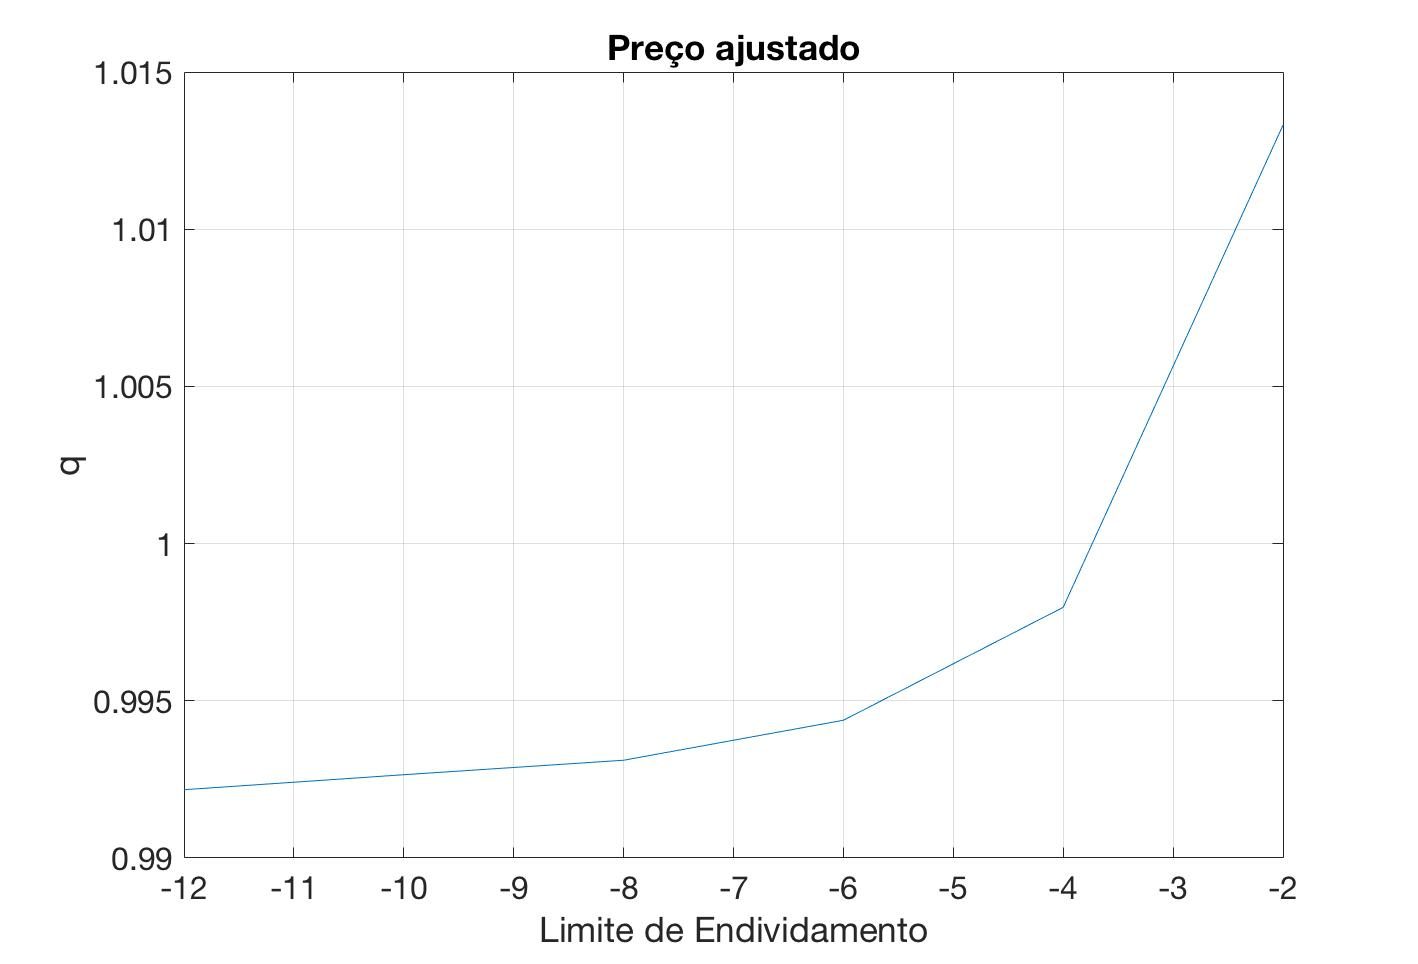
\includegraphics[scale = 0.25]{preco_ajustado}
\end{center}

\section*{Exerc�cio 2}

O arquivo \textit{q2.m} cont�m o c�digo que usamos para reproduzir a tabela do paper em quest�o. Obtivemos os seguintes resultados:

\begin{figure}[h!]
	\centering
	\begin{subfigure}{.5\textwidth}
		\centering
		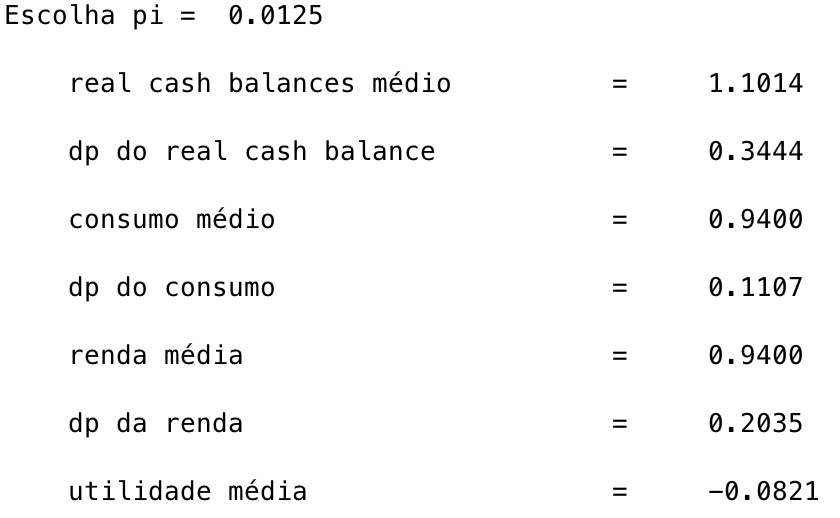
\includegraphics[scale = 0.5]{pi_125}
	\end{subfigure}%
	\begin{subfigure}{.5\textwidth}
  		\centering
  		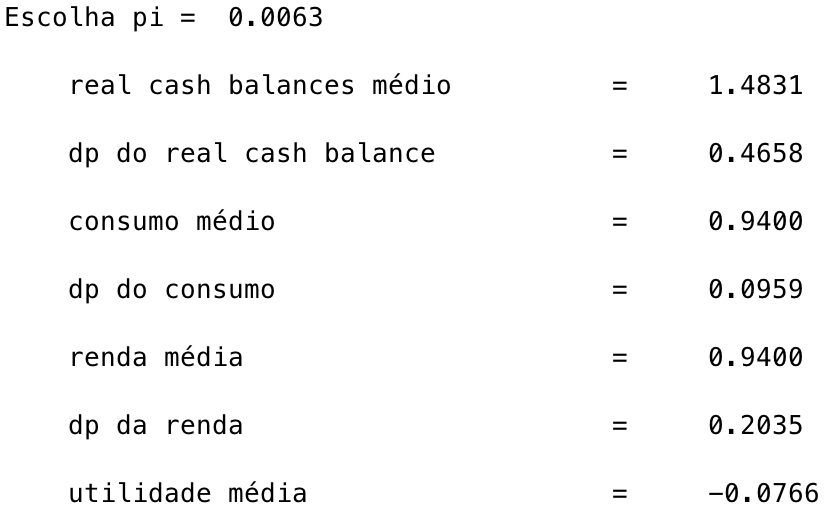
\includegraphics[scale = 0.5]{pi63}
  	\end{subfigure}
  	
  	\vspace{0.5cm}
  	
  	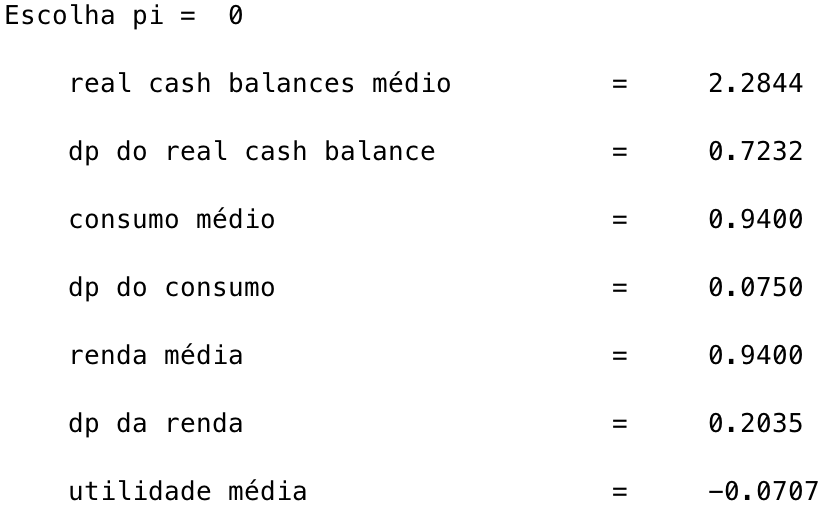
\includegraphics[scale = 0.5]{pi0}
\end{figure}

\section*{Exerc�cio 3}
	

\end{document}